\section{Ejercicio 4}

%SI QUIEREN AGREGAR IMAGENES COPIEN EL SIGUIENTE CODIGO
%\begin {center}
%\includegraphics[width=12cm]{./graphEj1.jpg}
% grafico.eps: 0x0 pixel, 300dpi, 0.00x0.00 cm, bb=50 50 410 302
%\end {center}


En el siguiente gráfico se puede observar el diagrama de Gantt para el lote LoteEj4.tsk ejecutadas mediante el scheduler Round-Robin con un quantum igual 11.

\begin {center}
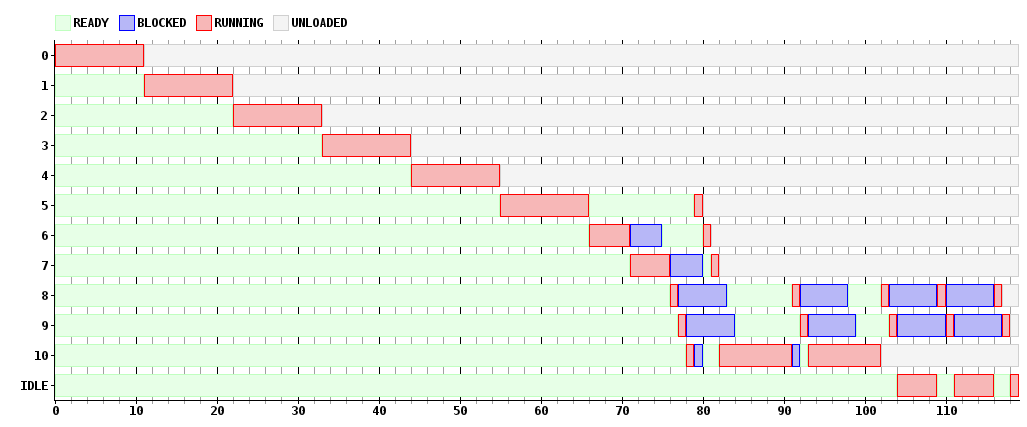
\includegraphics[width=12cm]{../simusched/outputs/outEj4.png}
 grafico.eps: 0x0 pixel, 300dpi, 0.00x0.00 cm, bb=50 50 410 302
\end {center}

Descripción del diagrama:
En la ejecución de las primeras 5 tareas se parece al scheduler FIFO, debido a que puede ejecutarlas enteras en 1 solo Quantum. Pero a partir de la quinta tarea podemos observar el funcionamiento del Round-Robin en todo su esplendor.
La tarea numero 5 se ejecuta durante 11 ciclos y antes de ser finalizada el scheduler la saca y pone a la siguiente debido a que se termino su 'tiempo' (llego a los 11 ciclos, es decir alcanzo el quantum).
La tarea numero 6 se ejecuta durante 4 cilcos y luego se bloquea durante otros 4 utlizando un cilco extra para llamar a la ejecución de la llamada. Cuando esta tarea procede a bloquearse el scheduler (a diferencia del FIFO) cambia a la tarea siguiente y esta procede de la misma manera.
Las 2 tareas siguientes se comportan muy parecido nada mas que lo primero que hacen es bloquearse y por lo tanto el scheduler las deja solo 1 ciclo en ejecucion.
Por último la tarea 10 también realiza un bloqueo apenas se ejecuta por una cuestion aleatoria (la tarea 10 es la taskBatch y el momento en que ejecuta el bloqueo es aleatorio).
Luego de haber ejecutado lo correspondiente a todas las tareas vuelve a la numero 5 (que no habia sido terminada de ejecutar), una vez que esta termina, cambia a la siguiente (aunque no se haya cumplido el quantum, si no desperdiciarian ciclos).Lo mismo sucede con las dos tareas siguientes.
Como la tarea numero 8 sigue bloqueada, no la ejecuta al igual que la tarea 9.
Carga la tarea 10 hasta que esta se vuelve a bloquear y la cambia por la tarea 8 (que ya no se encuentra bloqueada) esta bloquea y repite el procedimiento para la tarea 9. 
Termina de ejecutar la tarea 10 y aca podemos observar que hay un momento en que si bien las tareas 8 y 9 son las unicas tareas cargadas no finalizadas aún no las carga debido a que se encuentran bloqueadas y por eso se corre la tarea IDLE hasta que se desbloquea alguna de las 2.
Finalmente repite esa ultima secuencia 1 vez mas y finaliza la ejecución de todas las tareas.

Resumen:
A diferencia del FIFO este scheduler no (necesariamente) ejecuta una tarea hasta que esta finalize, sino que hasta que se cumpla el Quantum de ciclos, el proceso se bloquee o efectivamente concluya. Por otro lado también cabe enfatizar que el orden en que las alterna esta dado por una cola en la que las tareas se encuentran ordenandas por orden llegada, donde una vez ejecutada la última vuelve a la primera no acabada y sólo ejecuta la tarea idle en caso que el resto de las tareas se encuentren bloqueadas.
Finalmente este scheduler es mas óptimo (en comparación al FIFO) cuando se desea realizar la sensación de que se está ejecutando todo en simulteaneo (multiprogramación), obviamente con un rango de quantum tal qué sea imperceptible para el usuario y hace un mejor uso del cpu ya que cuando una tarea se encuentra bloqueada la quita y pone a otra tarea que este en estado "ready" para no desperdiciar ciclos de ejecución.
